\documentclass[a4paper]{article}
\usepackage[margin=1in]{geometry} 
% \usepackage{ctex}
\usepackage{tabularx}
\usepackage{lipsum}
\usepackage{enumerate}
\usepackage{amsfonts}
\usepackage{amsmath}
\usepackage{multirow}
\usepackage{graphicx}
% \usepackage{aligned}

\begin{document}
\begin{titlepage}
    \title{\textbf{Lab Report 2: Investigating the relationship between horizontal displacement and falling distance in projectile motion.}}
    \author{Eric Zhou}
    \date{\today}
    \maketitle
    %\tableofcontents
\end{titlepage}

\section{Raw data}

Diameter of the ball $d' = 1.580 \pm 0.005 cm$

\begin{table}[h]
    \centering
    \begin{tabular}{lllll}
        \hline
        \textbf{Trial} & \textbf{Photogate passing time $t(ms)$} & \textbf{Height $h(cm)$} & \multicolumn{2}{l}{\textbf{Horizontal displacement $d(cm)$}} \\ \hline
        1              & $17.13 \pm 0.01$                        & $77.7 \pm 0.5$          & $33.7 \pm 0.5$                & $33.4 \pm 0.5$               \\
        2              & $17.80 \pm 0.01$                        & $40.2 \pm 0.5$          & $23.2 \pm 0.5$                & $23.3 \pm 0.5$               \\
        3              & $17.17 \pm 0.01$                        & $31.8 \pm 0.5$          & $20.2 \pm 0.5$                & $20.6 \pm 0.5$               \\
        4              &                                         & $28.6 \pm 0.5$          & $19.6 \pm 0.5$                & $19.1 \pm 0.5$               \\
        5              &                                         & $26.3 \pm 0.5$          & $19.3 \pm 0.5$                & $19.6\pm 0.5$                \\ \hline
    \end{tabular}
    \caption{Raw data}
\end{table}

\section{Processed data}

Average photogate passing time $\bar{t} = 17.37 (\pm 1.93\%) ms$.

Initial velocity $v = {1.580 \over 17.37} = 0.091 cm/ms = 0.91m/s$.

Velocity error $\Delta v =\pm (1.93\% + 0.32\%) v =\pm 0.02m/s$.

\begin{table}[h]
    \centering
    \begin{tabular}{lllll}
    \hline
    \textbf{Trial} & \textbf{Avg. horizontal disp. $\bar{d} (cm)$} & \textbf{Error $\Delta \bar{d} (\%)$} & \textbf{Height squared $d^2(cm^2)$} & \textbf{Error $\Delta d^2(cm^2)$} \\ \hline
    1              & 33.55                             & 0.44                                 & $1125.6025$                         & $10.065$                        \\
    2              & 23.25                             & 0.21                                 & $540.5625$                          & $2.325$                         \\
    3              & 20.5                              & 0.48                                 & $420.25$                            & $4.1$                           \\
    4              & 19.35                             & 1.29                                 & $374.4225$                          & $9.675$                         \\
    5              & 19.45                             & 0.77                                 & $378.3025$                          & $5.835$                         \\ \hline
    \end{tabular}
    \caption{Processed data}
\end{table}

\section{Sample working}

Take the wroking process of trial $1$ data as an example. We can find 

\begin{equation}
    \begin{aligned}
        &\bar{d} = {{d_1 + d_2} \over 2} = {{33.7cm + 33.4cm} \over 2} = 33.55cm \\
        &\Delta\bar{d} = \pm{{|d_1 - d_2|}\over 2} = \pm{{33.7cm - 33.4cm} \over 2} = \pm0.15cm \\
        &\%\Delta\bar{d} = {{\Delta\bar{d}}\over \bar{d}} = \pm 0.44\%  \\
        &\bar{d} ^2 = 1125.6025cm \\
        &\%\Delta(\bar{d}^2) = 2\%\Delta\bar{d} = \pm 0.88\% \\
        &\Delta(\bar{d}^2) = 0.88\% \times \bar{d} ^2 = \pm 10.065cm
    \end{aligned}
\end{equation}

Where $\bar{d}$ is the average value of $d$, $\%\Delta$ refers to the percentage uncertainty of the following variable and $\Delta$ refers to the absolute uncertainty of the following value.

\section{Diagram}

$\bar{d}^2$ alongside with its error is plotted against $h$, the graph plotted is shown in Figure \ref{fig.d2-h}.

\begin{figure}[h]
    \centering
    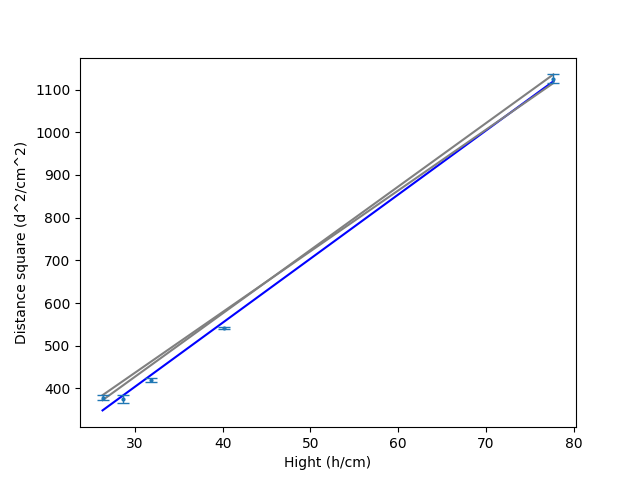
\includegraphics[width = 0.8\textwidth]{Figure_1.png}
    \caption{$d^2 - h$ graph}
    \label{fig.d2-h}
\end{figure}

Linear fit is used to find the relationship between $d^2$ and $h$. A linear fit of $15.00h - 46.06 = d^2$ is found. 

\section{Analysis and conclusion}

We can find in our previous hypothesis that

\begin{equation}
    \begin{aligned}
        & d^2 = {{2v_0^2}\over g}h
    \end{aligned}
\end{equation}

as $d$ and $h$ are in centimeter, ${2v_0^2}\over g$ should be $0.1500m$. 

According to our measurement of $d'$, the measured ${{2v_0^2}\over g}$ is $0.169 \pm 0.008m$.

The calculated value shows a percentage error of ${|0.15 - 0.161|\over 0.161} = 6.83\%$. This is an error within a reasonable range.

\end{document}